% -----------------------------*- LaTeX -*------------------------------
\documentclass[12pt]{report}
\usepackage{%
	amsfonts,%
	amsmath,%	
	amssymb,%
	amsthm,%
	algorithm,%
	babel,%
	bbm,%
	etex,%
	%biblatex,%
	caption,%
	centernot,%
	color,%
	dsfont,%
	enumerate,%
	epsfig,%
	epstopdf,%
	geometry,%
	graphicx,%
	hyperref,%
	latexsym,%
	mathtools,%
	multicol,%
	pgf,%
	pgfplots,%
	pgfplotstable,%
	pgfpages,%
	proof,%
	psfrag,%
	subfigure,%	
	tikz,%
	ulem,%
	url%
}	
\usepackage[noend]{algpseudocode}
\usepackage[mathscr]{eucal}
\usepgflibrary{shapes}
\usetikzlibrary{%
  	arrows,%
	backgrounds,%
	chains,%
	decorations.pathmorphing,% /pgf/decoration/random steps | erste Graphik
	decorations.text,%
	matrix,%
  	positioning,% wg. " of "
  	fit,%
	patterns,%
  	petri,%
	plotmarks,%
  	scopes,%
	shadows,%
  	shapes.misc,% wg. rounded rectangle
  	shapes.arrows,%
	shapes.callouts,%
  	shapes%
}

\theoremstyle{plain}
\newtheorem{thm}{Theorem}[section]
\newtheorem{lem}[thm]{Lemma}
\newtheorem{prop}[thm]{Proposition}
\newtheorem{cor}[thm]{Corollary}

\theoremstyle{definition}
\newtheorem{defn}[thm]{Definition}
\newtheorem{conj}[thm]{Conjecture}
\newtheorem{exmp}[thm]{Example}
\newtheorem{assum}[thm]{Assumptions}
\newtheorem{axiom}[thm]{Axiom}

\theoremstyle{remark}
\newtheorem{rem}{Remark}
\newtheorem{note}{Note}
\newtheorem{fact}{Fact}

\newcommand{\norm}[1]{\left\lVert#1\right\rVert}
\newcommand{\indep}{\!\perp\!\!\!\perp}
\DeclarePairedDelimiter\abs{\lvert}{\rvert}%
\newcommand\numberthis{\addtocounter{equation}{1}\tag{\theequation}}
\newcommand{\tr}{\operatorname{tr}}
\newcommand{\R}{\mathbb{R}}
\newcommand{\N}{\mathbb{N}}
\newcommand{\E}{\mathbb{E}}
\newcommand{\Z}{\mathbb{Z}}
\newcommand{\B}{\mathscr{B}}
\newcommand{\C}{\mathcal{C}}
\newcommand{\T}{\mathscr{T}}
\newcommand{\F}{\mathcal{F}}
\newcommand{\G}{\mathcal{G}}
%\newcommand{\ba}{\begin{align*}}
%\newcommand{\ea}{\end{align*}}
\DeclareMathOperator*{\argmax}{arg\,max}
\renewcommand{\qedsymbol}{$\blacksquare$}
\makeatletter
\def\BState{\State\hskip-\ALG@thistlm}
\makeatother

\makeatletter
\def\th@plain{%
  \thm@notefont{}% same as heading font
  \itshape % body font
}
\def\th@definition{%
  \thm@notefont{}% same as heading font
  \normalfont % body font
}
\makeatother
\date{}
\usepackage{scribe_e1244}
\usepackage{times}
\begin{document}

% \course{CS 497}			% optional
% \coursetitle{Geometric Data Structures} % optional
% \semester{Fall 1998}			% optional
\lecturer{Aditya Gopalan}		% optional, put lecturer's name here
\scribe{Aditya Gopalan}		% required, put your name here
\lecturenumber{1}			% required, must be a number
\lecturedate{September 3}		% required, omit year
\maketitle

% title of the lecture
\begin{center}
{\Large \bf Introduction to Hypothesis Testing --\\ Bayesian Hypothesis Testing}
\end{center}

% ----------------------------------------------------------------------

\section{Administrative details}
\begin{itemize}
\item {\bf Instructors:} Aditya Gopalan (aditya@ece.iisc.ernet.in), Parimal Parag (parimal@ece.iisc.ernet.in)
\item {\bf Teaching assistant:} Raghava GD (raghavagd@ece.iisc.ernet.in)
\item {\bf Grading policy:} Homework assignments (including programming exercises): 30\%, Scribing lectures: 10\%, Midterm exam: 20\%, Final exam: 40\%
\item {\bf Course webpage:} {\tt www.ece.iisc.ernet.in/$\sim$parimal/estimation.html}
\item {\bf Scribing:} Administered via Github, sign up via course webpage/email
\item {\bf Course discussions:} Administered via Slack, sign up via course webpage/email
\item {\bf Texbooks:} V. Poor \cite{Poor}, Casella \& Berger \cite{CaseBerg:01} (also on the course webpage)
\end{itemize}

\section{Introduction}
\subsubsection{Detection}
Detection, broadly speaking, is the process of answering the question ``Is $\mathbf{X}$ present (or not)?", based on observations or data. $\mathbf{X}$ is a property of interest. \\

\noindent Examples:
\begin{itemize}
\item (Communication systems) Is there a message that was sent (based on received data)?
\item (Radar) Is there an enemy airplane in the vicinity?
\item (Astronomy) Is there a planet/star/nebula in this part of space?
\item (Medicine) Is this patient sick? Is treatment $\mathbf{T}$ effective for disease $\mathbf{D}$?
\item (Physics) Is this body hot/massive/dense? Is the Higgs boson present?
\item (Economics) Is there a slowdown in economic growth since November 8, 2016 \cite{Hin16:demonetization}?
\end{itemize}

\subsubsection{Estimation}
Estimation is the process of answering the question ``What is the value $\mathbf{X}$?", based on observations or data. $\mathbf{X}$ is typically a quantity of interest. \\

\noindent Examples:
\begin{itemize}
\item (Communication systems) What is the message that was sent? What was the temperature measurement from the sensor when it was transmitted to the processor?
\item (GPS) What is my position/velocity/acceleration?
\item (Astronomy) What is the size of the planet? What is its chemical composition?
\item (Economics) What is India's GDP/population size today? What was the typical waiting time to withdraw cash from ATMS on November 8, 2016 \cite{Hin16:demonetization}?
\end{itemize}

\subsection{Goals of this course and takeaways}
\begin{enumerate}
\item Study the qualitative problems of detection and estimation in the framework of {\bf statistical inference}.
\item Gain an understanding of, and develop the ability to design, automated systems for detection and estimation (these are often key subsystems of larger systems in real life). 
\end{enumerate}

\section{Detection theory}

We frame problems of detection in the language of {\em statistical hypothesis testing} [K. Pearson, W. S. Gosset, R. Fisher, J. Neyman, E. Pearson, pre- and post- World War II period]. 

\subsection{The hypothesis testing framework}
\begin{itemize}
\item $\Gamma$: Observation set
\item $\mathcal{G}$: Class of subsets of $\Gamma$ that can be assigned probabilities. We will typically take this to be a $\sigma$-algebra, i.e., a class of subsets containing $\emptyset$ and $\Gamma$, and closed under complements and countable unions. Examples: (a) $\Gamma = \{1, 2, \ldots, n\} \equiv [n]$, $\mathcal{G} = 2^\Gamma$, the power set (all subsets) of $\Gamma$, (b) $\Gamma = \mathbb{R}$, $\mathcal{G} = \mathcal{B}(\mathbb{R})$, the Borel $\sigma$-algebra on $\mathbb{R}$.

\item {\bf Notation.} $\prob{A}$: the probability assigned to $A \subseteq \Gamma$, $\indic{\mathbf{X}}$: the indicator function (1 if true, 0 if false) of $\mathbf{X}$
\end{itemize}

\noindent {\em $M$-ary hypothesis testing:} Decide which of $M$ possible situations could describe the situation at hand, based on an observation $Y \in \Gamma$. \\

The case $M = 2$ is important and known as {\em binary hypothesis testing}, and will form the focus of our study for several classes. 

\subsection{Binary hypothesis testing}
We assume that there are two possible hypotheses, $H_0$ and $H_1$, which correspond to two probability distributions $\mathbb{P}_0$ and $\mathbb{P}_1$, respectively, on $(\Gamma, \mathcal{G})$. \\

{\em Problem}: Decide \noindent $H_0: Y \in \Gamma, Y \sim \mathbb{P}_0$ (the ``null" hypothesis) vs. \noindent $H_1: Y \in \Gamma, Y \sim \mathbb{P}_1$ (the ``alternative" hypothesis)

\begin{defn}
A decision rule (or hypothesis test) for $H_0$ vs $H_1$ is a map $\delta: \Gamma \to \{0, 1\}$.
\end{defn}

Equivalently, a decision rule is a {\em partition} of the observation space $\Gamma$ into two regions, corresponding to deciding $H_0$ or $H_1$ (Figure \ref{fig:decrule}):
\begin{align*}
\Gamma_0 &\bydef \{y \in \Gamma: \delta(y) = 0\}, \\
\Gamma_1 &\bydef \{y \in \Gamma: \delta(y) = 1\}. 
\end{align*}
{\em Note:} We have the identity $\delta(y) = \indic{y \in \Gamma_1}$ $\forall y \in \Gamma$. \\

\begin{figure}[htbp]
\begin{center}
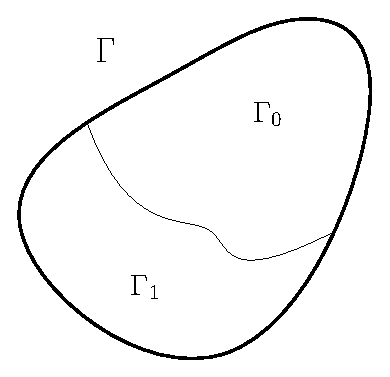
\includegraphics[scale = 0.8]{Figures/Gamma.eps}
\caption{A decision rule $\delta$ in terms of its partition of the observation space.}
\label{fig:decrule}
\end{center}
\end{figure}

\noindent {\em Cost}: We denote by $C_{i,j}$ the cost of deciding hypothesis $H_i$ when hypothesis $H_j$ was actually true, $i, j \in \{0,1\}$. Typically, $C_{ij} \approx 0$ if $i = j$ and $C_{ij} \gg 0$ otherwise.

\begin{defn}
The {\em conditional risk} of a decision rule $\delta$ for hypothesis $j \in \{0,1\}$ is its expected cost when hypothesis $j$ is actually true. We denote it by $R_j(\delta)$. Thus, 
\begin{align*}
R_j(\delta) &\bydef \mathbb{E}_j\left[ C_{j0}\indic{Y \in \Gamma_0} + C_{j1}\indic{Y \in \Gamma_1} \right] \\
&= C_{j0} \, \mathbbm{P}_j[\Gamma_0] + C_{j1} \, \mathbbm{P}_j[\Gamma_1].
\end{align*}
\end{defn}

There are several ways of defining the performance of decision rules. The first one we will study is within a Bayesian setting.

\subsection{Bayesian (binary) hypothesis testing}
\begin{assum}
There are known {\em prior} or {\em a priori} probabilities of the occurrences of hypotheses $H_0$ and $H_1$, denoted by $\pi_0$ and $\pi_1$, respectively (note: $\pi_0 + \pi_1 = 1$).
\end{assum}

\begin{defn}
The {\em Bayes risk} of a decision rule $\delta$, denoted by $r(\delta)$, is the average cost incurred by $\delta$ under the prior distribution $(\pi_0, \pi_1)$, i.e., $r(\delta) \bydef \pi_0 R_0(\delta) + \pi_1 R_1(\delta)$.
\end{defn}

\begin{defn}
An optimal rule for Bayesian hypothesis testing is a rule $\delta$ that minimizes $r(\delta)$. We also call such a rule a {\em Bayes rule} (not to be confused by Bayes' formula in probability!). 
\end{defn}

\subsubsection{Finding a Bayes rule}

For a decision rule $\delta$, we have
\begin{align*}
r(\delta) &\bydef \pi_0 R_0(\delta) + \pi_1 R_1(\delta) \\
&= \sum_{j=0}^1 \pi_j R_j(\delta) \\
&= \sum_{j=0}^1 \pi_j \left( C_{j0} \, \mathbbm{P}_j[\Gamma_0] + C_{j1} \, \mathbbm{P}_j[\Gamma_1] \right) \\
&= \sum_{j=0}^1 \pi_j \left( C_{j0} \, \left(1 -  \mathbbm{P}_j[\Gamma_1] \right) + C_{j1} \, \mathbbm{P}_j[\Gamma_1] \right) \\
&= \sum_{j=0}^1  \pi_j \, C_{j0}  + \sum_{j=0}^1 \pi_j \left( C_{j1} - C_{j0} \right) \mathbbm{P}_j[\Gamma_1]. 
\end{align*}
Let us assume for concreteness that the probability distribution $\mathbbm{P}_j$ has a probability density function (pdf) or probability mass function (pmf) $p_j$ (most cases we will encounter will have one of these properties). We can continue thus: 
\begin{align*}
r(\delta) &= \sum_{j=0}^1  \pi_j \, C_{j0}  + \sum_{j=0}^1 \pi_j \left( C_{j1} - C_{j0} \right) \int_{\Gamma_1}p_j(y) dy \\
&= \sum_{j=0}^1  \pi_j \, C_{j0}  + \sum_{j=0}^1 \pi_j \left( C_{j1} - C_{j0} \right) \int_{\Gamma} \delta(y) \, p_j(y) dy \\
&= \sum_{j=0}^1  \pi_j \, C_{j0}  + \int_{\Gamma} \left[ \sum_{j=0}^1 \pi_j \left( C_{j1} - C_{j0} \right) p_j (y) \right]  \delta(y) dy.
\end{align*}
Therefore, the best choice of $\delta: \Gamma \to \{0,1\}$, to minimize $r(\delta)$, is to set $\delta(y) = 1$ if and only if the integrand in square brackets in the above expression is nonpositive. In other words, {\em the following rule $\delta_B$ is a Bayes rule}:
\[ \delta_B(y) = \left\{ 
\begin{array}{cc}
1, &  \text{if }\sum_{j=0}^1 \pi_j \left( C_{j1} - C_{j0} \right) p_j (y) \leq 0 \\
0, &  \text{if }\sum_{j=0}^1 \pi_j \left( C_{j1} - C_{j0} \right) p_j (y) > 0. \\
\end{array}
 \right. \]
 (Note: Breaking ties either way does not change the Bayes risk and is thus inconsequential as far as Bayes optimality is concerned.)


\bibliography{Lecture_01_Scribe_Notes}
\bibliographystyle{IEEEtran}
\end{document}

